\chapter{Topología de Espacios métricos}
	\section{Conjuntos abiertos y cerrados}
	\begin{nota}
		Sea $(M,d)$ un espacio m\'etrico recordamos que si $N\subset M$ entonces $(N,d|_{_{N\times N}})$ es un espacio m\'etrico.
	\end{nota}
	
	\begin{defi} Sea $a\in M $ y $r>0$
		\begin{itemize}
			\item $B(a,r)= \{ x\in M\talque d(x,a)<r\}$ \underline{Bola abierta de centro $a$ y radio 				$r$.}
			\item $\overline{B}(a,r)=\{ x\in M\talque d(x,a)\leq r\}$ \underline{Bola cerrada de centro $a$ y radio $r$.}
		\end{itemize}
	\end{defi}
	
	\begin{defi} Sea $(M,d)$ y sea $A \subset M$ decimos que:
		\begin{itemize}
			\item \underline{$A$ es abierto} si $\forall a \in A \ \exists r>0\talque B(a,r) \subset A$
			\item \underline{$A$ es cerrado} si $A^c(=M\setminus A)$ es abierto.
			\item Sea $a\in M$, decimos que \underline{$U\subset M$ es entorno de $a$} si $\exists r>0\ | 				\ B(a,r) \subset U$
		\end{itemize}
	\end{defi}
	
	\begin{proposicion}
		$A$ es abierto $\iff \ A$ es entorno de $a,\ \forall a \in A$
	\end{proposicion}
	
	\begin{proposicion}Propiedades de los subconjuntos abiertos de $M$
		\begin{enumerate}[1)]
 			\item $M,\ \emptyset$ Son abiertos.
 			\item La uni\'on de abiertos es abierta.
 			\item La intersecci\'on de una familia \underline{finita} de abiertos es un subconjunto 						abierto.
		\end{enumerate}
	\end{proposicion}

	\begin{corolario} Por las leyes de Morgan obtenemos las siguientes propiedades de subconjuntos cerrados de $M$:
 		\begin{enumerate}[1)]
			\item $M,\ \emptyset$ Son cerrados.
			\item La intersecci\'on de cerrados es cerrada.
			\item La uni\'on de una familia \underline{finita} de cerrados es un subconjunto cerrado.\\
	 	\end{enumerate}
 	\end{corolario}
 	
 	\section{Topología básica}
 	
 	\begin{defi} Sea $A\subset M$ y sea $x\in M$
		\begin{itemize}
			\item Decimos que $x$ es \underline{punto interior} de $A$ si $\exists r>0\talque B(x,r)\subset A$
			\item Decimos que $x$ es \underline{punto de acumulaci\'on} de $A$ si $\forall r>0\talque (B(x,r)-\{ x\}\cap A) \neq \emptyset$
			\item Decimos que $x$ es \underline{punto adherente} de $A$ si $\forall r>0\talque B(x,r)\cap A \neq \emptyset$
			\item Decimos que $x$ es \underline{punto frontera} de $A$ si \[\forall r>0\
\left\{
	      	\begin{array}{ll}
		 B(x,r)\cap A \neq \emptyset \\
		 B(x,r)\cap A^c \neq \emptyset \\
	       \end{array}
	     \right.\]
	    	\item Decimos que $x$ es \underline{punto aislado} de $A$ si $\exists r>0\talque B(x,r)\cap A = \{x\}$		
			\item Decimos que $x$ es \underline{punto exterior} de $A$ si $\exists r>0\talque B(x,r)\subset A^c$
		\end{itemize}
	
		\begin{enumerate}[-]
			\item $\mathring{A}=$ puntos interiores de $A$
			\item $A'=$ puntos de acumulaci\'on de $A$
			\item $\overline{A}=$ puntos adherentes de $A$
			\item $\fr(A)=$ puntos frontera de $A$
			\item $\ais(A)=$ puntos aislados de $A$
		\end{enumerate}
	\end{defi}	
	
	\begin{proposicion}\ 
		\begin{enumerate}[1)]
			\item $\mathring{A}$ es el mayor abierto contenido en $A$ 
				\begin{align*}
					\mathring{A} =\cup\{ G \subset M\talque G \mathrm{\ es\ abierto\ y\ } G\subset A\}
				\end{align*}
			\item $\overline A$ es el menor cerrado que contiene a $A$
				\begin{align*}
					\overline A=\cap\{F\subset M\talque F \mathrm{\ es\ cerrado\ y\ } A\subset F\}
				\end{align*}
		\end{enumerate}
	\end{proposicion}
	
	\begin{proposicion} \ 
		\begin{itemize}
			\item $A$ es abierto $\iff A = \mathring{A}$
			\item $A$ es cerrado $\iff A =\overline{A}$ \\
		\end{itemize}
	\end{proposicion}
	
	\begin{nota}Ser ``abierto'' o ``cerrado'' dependen del espacio ambiente.
		\begin{ejem} $(0,1]$ es cerrado en $\mathbb{R}^+$ y no lo es en $\mathbb{R}$\\
		\end{ejem}
	\end{nota}
	
	\begin{proposicion} \ 
		\begin{itemize}
			\item $\overline{A}= A\cup \fr(A)=A\cup A'=\ais(A)\cup A'$
			\item $\fr(A)=\overline{A}\setminus\mathring{A}$
		\end{itemize}
	\end{proposicion}	
	
	\begin{defi}Una m\'etrica $d$ en un conjunto $M$ genera una topolog\'ia que es la colecci\'on de los conjuntos abiertos. La denotamos as\'i:
	\[\tau_d=\{A\subset M\talque A \mathrm{\ es\ abierto}\}\]
	\end{defi}
	
	\begin{defi} Sean $d_1$ y $d_2$ m\'etricas en un conjunto $M$, diremos que son 				 					\underline{equivalentes} si generan la misma topolog\'ia; es decir:
		\[\tau_{d_1}=\tau_{d_2}\]
	\end{defi}
	
	\begin{proposicion} Sean $d_1$ y $d_2$ m\'etricas en $M$, $d_1 \equiv d_2 \iff \ \forall x\in M, \ \forall r>0 \\ \exists\gamma_1>0\talque B_{d_1}(x,\gamma_1)\subset B_{d_2}(x,r)$ y $ \exists\gamma_2>0\talque B_{d_2}(x,\gamma_2)\subset B_{d_1}(x,r)$\\
	
	- Una condici\'on suficiente para que dos m\'etricas $d_1$ y $d_2$ en $M$ sean equivalentes es que $\exists c,C>0$ de manera que:
	\[cd_1(x,y)\leq d_2(x,y)\leq Cd_1(x,y)\ \forall x,y\in M\implies d_1\equiv d_2\] \\
	\underline{-Sin embargo esta condici\'on no es necesaria generalmente}\\
	-Si la m\'etricas $d_1$ y $d_2$ provienen de una norma, esta condici\'on se hace entonces \underline{necesaria} adem\'as de suficiente para que dichas m\'etricas sean equivalentes; es decir:
	\[\mathrm{Si\ }d_1,d_2\mathrm{\ provienen\ de\ una\ norma:\ }\]
	\[d_1\equiv d_2\iff \exists c,C>0 \talque cd_1(x,y)\leq d_2(x,y)\leq Cd_1(x,y)\ \forall x,y\in M\]
	\end{proposicion}	
	
	\begin{defi} Decimos que \underline{dos normas son equivalentes} en un espacio $E$ si $||\cdot||$ y $||\cdot||'$ generan la misma topolog\'ia.
	\end{defi}
	
	\begin{proposicion} $||\cdot||$ y $||\cdot||'$ son equivalentes $\iff \exists m,M>0$ tal que\\
	$m||x||\leq||x||'\leq M||x||\ \forall x\in E$
	\end{proposicion}
	\newpage
	\begin{ejem}
		En $(\mathbb{R}^2,d_2)$, sea $A=\{(x,y)\in \mathbb{R}^2\talque x>0,y>0,xy>1\}$ $A$ es abierto?\\
		
		En efecto $A$ es abierto:
		\begin{proof}		
			Probaremos que $\forall(a,b)\in A,\ \exists r>0\talque B((a,b),r)\subset A$
			\[\mathrm{Sabemos\ }  \left\{
				\begin{array}{ll}
					a>0 \\
			 		b>0 \\
					ab>1\\
		       \end{array}
		    \right\}\]
			\[\mathrm{Supongamos\ que\ }(x,y)\in B((a,b),r)\implies\{\sqrt{(x-a)^2+(y-b)^2}=d((x,y),(a,b))\}\implies \] \\
	\[\implies \left\{
	       \begin{array}{ll}
		 |x-a|<r \\
		 |y-b|<r \\
	       \end{array}
	     \right\}\implies \left\{
	       \begin{array}{ll}
		 a-r<x<a+r \\
		 b-r<y<b+r \\
	       \end{array}
	     \right\}\implies xy>(a-r)(b-r)=\] \\
	     \[=ab-r(a+b)+r^2>ab-r(a+b)\geq 1\iff ab-1\geq r(a+b)\iff\dfrac{ab-1}{a+b}\geq r>0\]
	     \[\mathrm{Por\ tanto\ para\ }0<r\leq \dfrac{ab-1}{a+b},\ xy>1.\mathrm{\ Veamos\ por\ ultimo\ que\ }x,y>0\]
	     \[ x>a-r\geq a-\dfrac{ab-1}{a+b}=\dfrac{a(a+b)-ab+1}{a+b}=\dfrac{a^2+1}{a+b}>0 \]
		 \[y>b-r\geq b-\dfrac{ab-1}{a+b}=\dfrac{b(a+b)-ab+1}{a+b}=\dfrac{b^2+1}{a+b}>0 \]
		\end{proof}
		\begin{figura}\ \\
	\begin{center}
	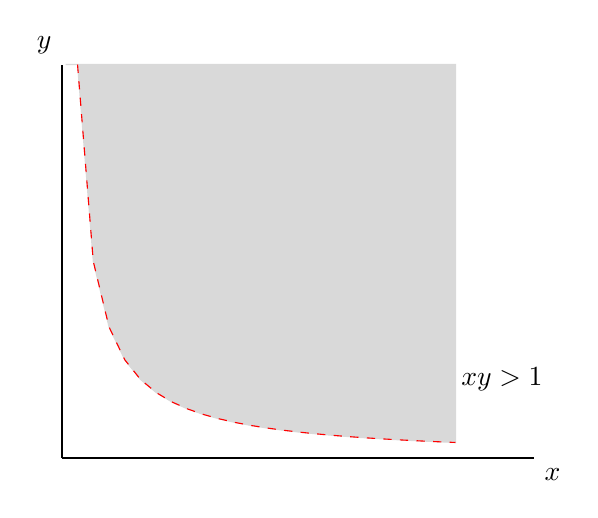
\begin{tikzpicture}
	\fill (4.95,1) circle (0.5pt)node[anchor=west] {$xy>1$};
	\filldraw[gray!30] plot [domain=0.05:5] ({\x},{5})
-- plot [domain=5:0.2] ({\x},{1/\x})
-- cycle;
		\draw[thick](0,0) -- (6,0) node[anchor=north west] {$x$};
		\draw[thick] (0,0) -- (0,5) node[anchor=south east] {$y$};
		\draw[domain=0.2:5,variable=\x,red,dashed] plot ({\x},{1/\x});
	\end{tikzpicture}
	\end{center}
	\end{figura}
	\end{ejem}